\section{Supplementary Dataset Examples and Structural Coverage}\label{app:contract}
\subsection{Examples from Original Schematic Windows}
Figures~\ref{fig:appendix1}--\ref{fig:appendix3} show six training examples drawn from six different original DWG windows, with no controlled wiring edits. None reuses a screenshot displayed in the main text. Questions and short answers retain the released wording; concise evidence summaries highlight the corresponding graph checks. These examples document dataset content, not model predictions or observed field faults. The examples retain their original source associations.

\begin{figure*}[p]
\centering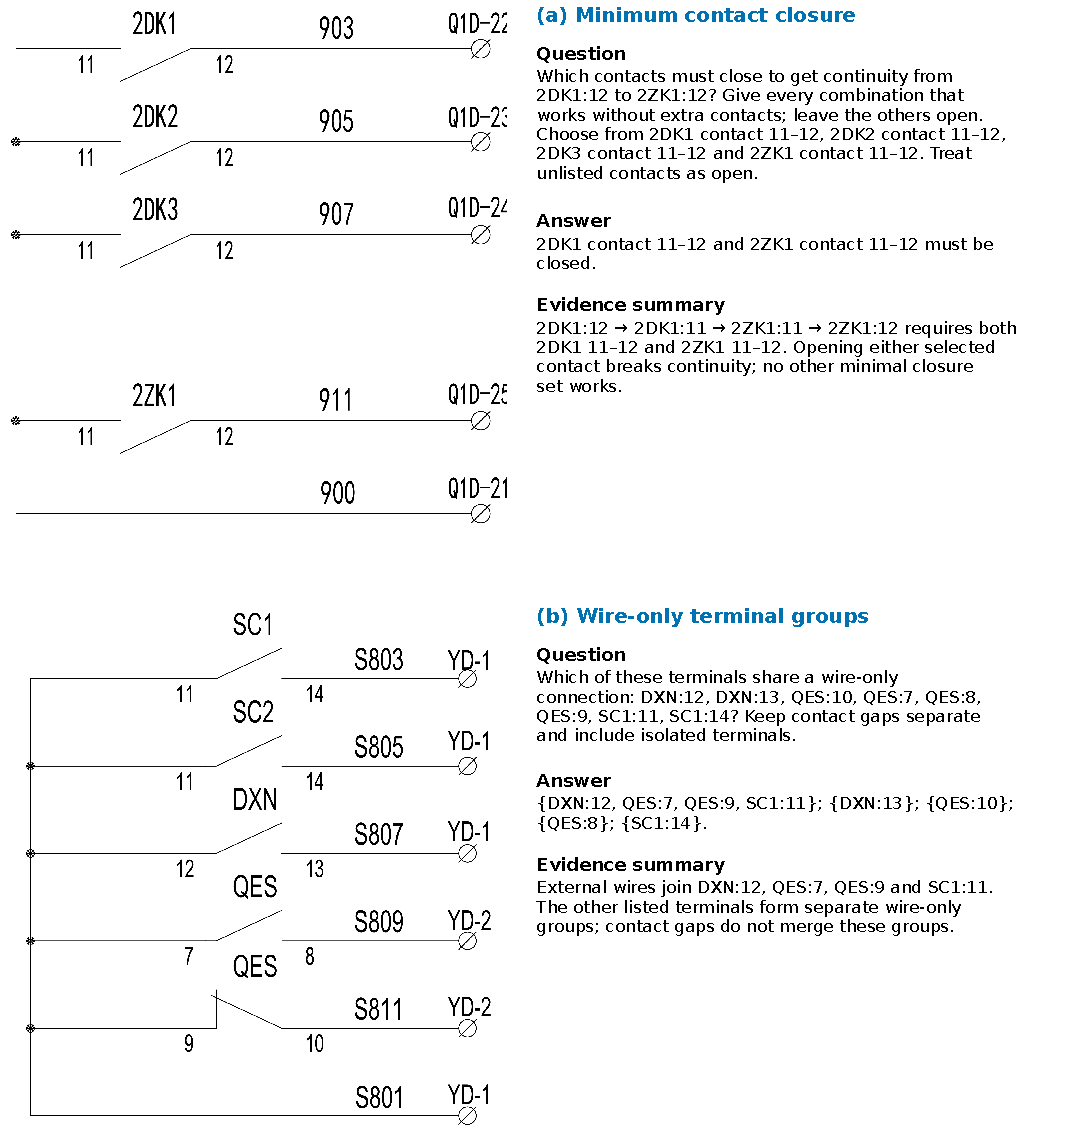
\includegraphics[width=.98\textwidth]{assets/figure_13.pdf}
\caption{Minimum contact closure and wire-only terminal grouping. Contact conduction is governed by the stated assumptions, whereas wire groups exclude contact edges.}
\label{fig:appendix1}
\end{figure*}

\begin{figure*}[p]
\centering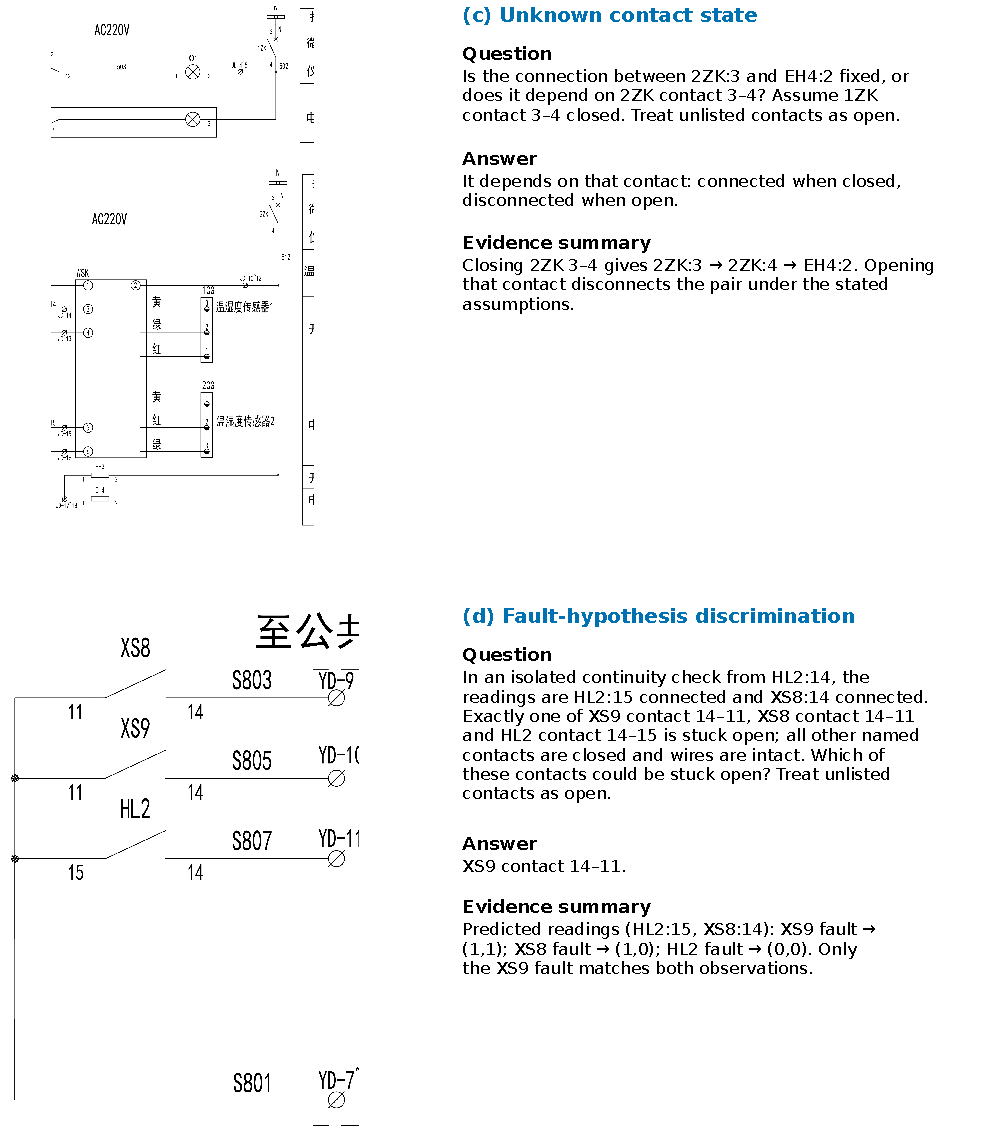
\includegraphics[width=.98\textwidth]{assets/figure_14.pdf}
\caption{State dependence and fault-hypothesis discrimination. Different contact states and fault hypotheses are checked against their corresponding continuity outcomes.}
\label{fig:appendix2}
\end{figure*}

\begin{figure*}[p]
\centering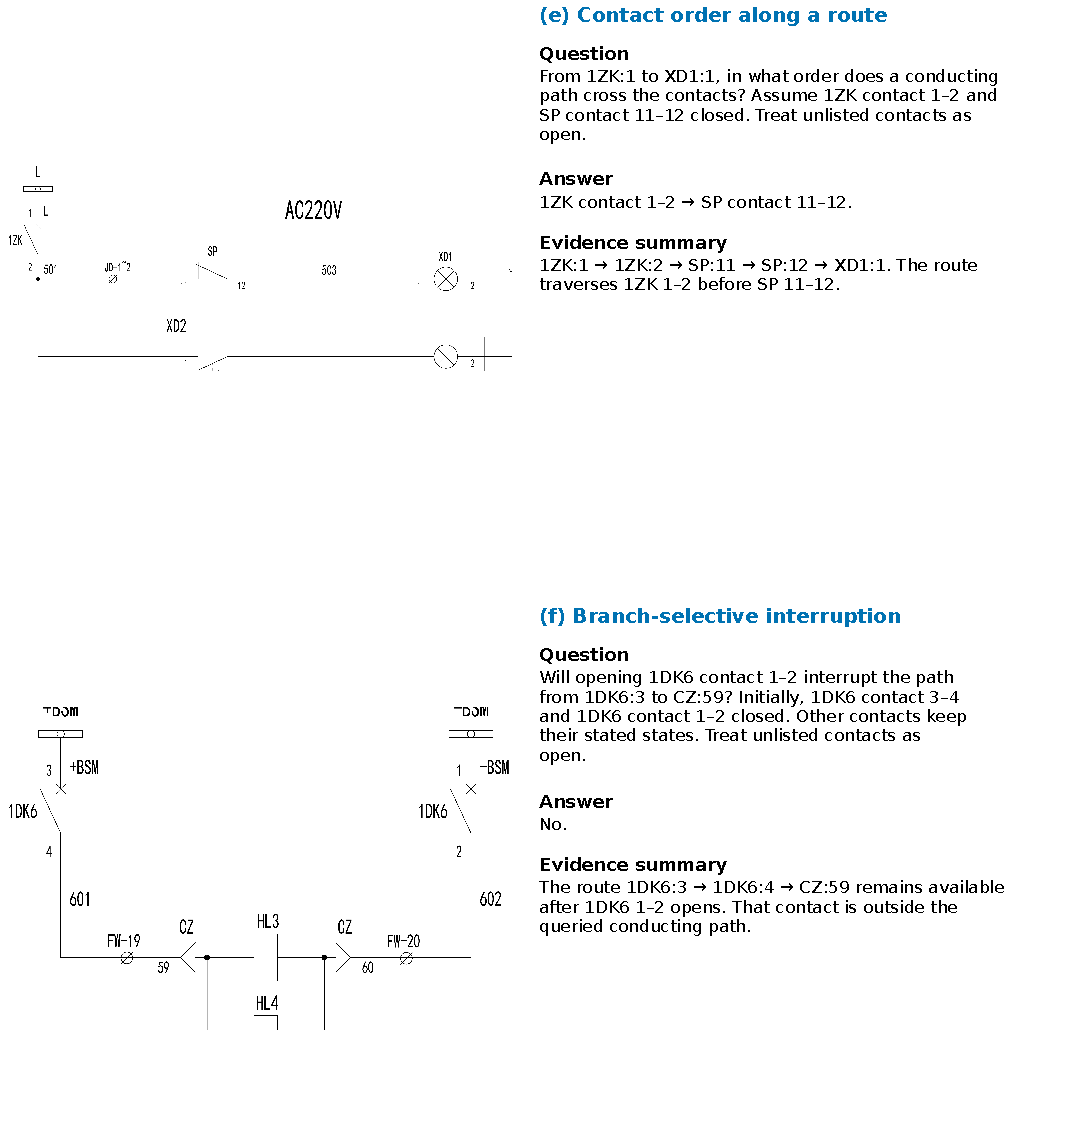
\includegraphics[width=.98\textwidth]{assets/figure_15.pdf}
\caption{Contact order and branch-selective interruption. A valid route identifies the traversed contacts; an unrelated contact opening leaves the queried branch connected.}
\label{fig:appendix3}
\end{figure*}

\subsection{Annotation and Evaluation Records}
Each annotation contains a question, short answer, compact evidence, typed result, task parameters, and source provenance. Verification queries store contact states, graph modifications, connectivity outcomes, and supporting paths or reachable regions. The two training views serialize the same image--question records with different supervision targets; they do not increase the number of distinct QA examples.

Answer and evidence quality are evaluated separately with a three-level electrical rubric. Unresolved judgments are retained, and joint correctness requires both dimensions to receive full credit for the same response.

\subsection{Structural Coverage and Pair Inventory}
Figure~\ref{fig:structure} summarizes the bounded reference graphs for the 300 original context windows, excluding edited variants. These are graph-level counts, not an inventory of every component visible in each screenshot. Table~\ref{tab:pairinventory} records the completed binary pair audit. The inventory is restricted to binary decisions with revalidated outcomes.

\begin{figure*}[t]
\centering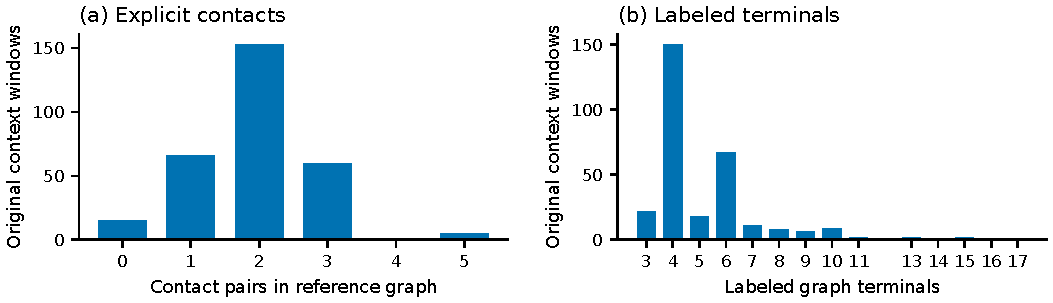
\includegraphics[width=.95\textwidth]{assets/figure_16.pdf}
\caption{Structural coverage of the bounded reference graphs in original contexts. Original windows may overlap within a drawing; graph statistics do not imply independent circuit designs.}
\label{fig:structure}
\end{figure*}

\begin{table}[t]
\centering\small\setlength{\tabcolsep}{3pt}
\caption{Revalidated binary pair inventory. Counts reuse existing QA and are not model scores.}
\label{tab:pairinventory}
\begin{tabularx}{\linewidth}{@{}Xrrrr@{}}\toprule
Split & Visual flip & Visual invariant & State flip & State invariant \\\midrule
Train & 79 & 178 & 340 & 283 \\
Validation & 13 & 23 & 37 & 58 \\
Test & 23 & 46 & 82 & 97 \\
\bottomrule\end{tabularx}
\end{table}
